\documentclass[conference]{IEEEtran}
\IEEEoverridecommandlockouts
\usepackage{cite}
\usepackage{amsmath,amssymb,amsfonts}
\usepackage{algorithmic}
\usepackage{graphicx}
\usepackage{textcomp}
\usepackage{xcolor}
\usepackage{booktabs}
\usepackage{url}
\def\BibTeX{{\rm B\kern-.05em{\sc i\kern-.025em b}\kern-.08em
    T\kern-.1667em\lower.7ex\hbox{E}\kern-.125emX}}
\graphicspath{{figures/}}

\begin{document}

\title{Fifteen Games Are Not a Season: Forecasting NBA Standings and Playoff Odds with Regularized Regression and Monte Carlo Simulation}

\author{\IEEEauthorblockN{[Author 1 Name]}
\IEEEauthorblockA{\textit{Federal University of ABC (UFABC)}\\
S\~ao Bernardo do Campo, Brazil \\
[email or RA]}
\and
\IEEEauthorblockN{[Author 2 Name]}
\IEEEauthorblockA{\textit{Federal University of ABC (UFABC)}\\
S\~ao Bernardo do Campo, Brazil \\
[email or RA]}
}

\maketitle

\begin{abstract}
After roughly fifteen games of an NBA regular season, the standings are dominated by noise, yet fans, media and teams already draw conclusions from them. We ask how well the final winning percentage of each team, and its probability of finishing in the top six, in the play-in zone or out of the postseason of its conference, can be predicted at that point of the 2026--27 season. Using sixteen seasons of team game logs collected with the nba\_api library, we build six features from the first fifteen games of each team and compare two naive baselines with ordinary least squares, Ridge, Lasso and random forest regressors under leave-one-season-out and temporal holdout validation. All learned models reduce the mean absolute error from 7.6 to about 5.6 wins on an 82-game scale; we select Ridge, whose penalty stabilizes nearly collinear point-based features without loss of accuracy. Feeding the Ridge forecasts into a logistic game model and simulating the remaining schedule 10,000 times yields probabilities that are well calibrated in an out-of-sample backtest, with 81\% coverage of nominal 80\% intervals.
\end{abstract}

\begin{IEEEkeywords}
sports analytics, ridge regression, regression to the mean, cross-validation, Monte Carlo simulation, basketball
\end{IEEEkeywords}

%=====================================================================
\section{Introduction}
Every November, a few NBA teams start far above or below expectations. Is a 14--3 start evidence of a contender, or a lucky streak that will fade? The question matters beyond fandom: front offices decide whether to buy or sell at the trade deadline, and media narratives form early. Statistically, it is a classic case of \emph{regression to the mean}: an early-season winning percentage is a noisy measurement of team strength, and extreme values tend to move back toward the league average~\cite{efron1975,efron1977}.

We study the following question: \emph{with about 15 games played in the 2026--27 NBA season, what will be the final winning percentage of each team, and what is the probability that each finishes in the top six (direct playoff spot), in the play-in tournament (7th--10th) or out, in its conference?}

Our approach has two stages. First, a supervised regression model maps information available after $N=15$ games to the final winning percentage. We frame this as a shrinkage problem, for which regularized linear models such as Ridge~\cite{hoerl1970} are a natural fit, and compare them with baselines, Lasso~\cite{tibshirani1996} and random forests~\cite{breiman2001}. Second, the predicted strengths feed a logistic game model and a Monte Carlo simulation~\cite{metropolis1949} of the remaining schedule, which turns point forecasts into probabilities of conference positions. We validate both stages out of sample, including a backtest of the full simulation on sixteen past seasons.

%=====================================================================
\section{Data}
\subsection{Source and collection}
We used the \texttt{LeagueGameLog} endpoint of the open-source \texttt{nba\_api} Python client~\cite{nbaapi}, which wraps the official \url{stats.nba.com} service, to collect team-level box scores of every regular-season game from 2010--11 to 2025--26 (16 complete seasons) and of the 2026--27 season up to November 22, 2026. Each team-game row contains the date, opponent, home or away indicator, result, points, field goal and free throw attempts, offensive rebounds and turnovers. Requests were spaced by one second, retried with exponential back-off on failure and cached as one CSV file per season. The remaining 2026--27 schedule (952 games) was obtained from the \texttt{ScheduleLeagueV2} endpoint. Franchise abbreviations that changed during the period (NJN$\to$BKN, NOH$\to$NOP) were normalized, and each team was mapped to its conference. The historical sample has 38{,}238 team-game rows (19{,}119 games).

\subsection{Unit of analysis and target}
Let $N$ be the smallest number of games played by any team in 2026--27 at collection time; here $N=15$ (teams had played 15 to 18 games). Each observation is a team-season (480 historical, 30 current). The target is the \emph{final winning percentage} $y$ rather than the number of wins, because three seasons were shortened (66 games per team in 2011--12, 64 to 75 in 2019--20 and 72 in 2020--21). Errors are reported in wins on an 82-game scale, i.e.\ $82\,|y-\hat y|$.

\subsection{Features}
All features are computed using only the first $N$ games of each team, so no information after a team's $N$-th game enters any feature:
\begin{itemize}
\item \textbf{Win \%} after $N$ games.
\item \textbf{Point differential per game}, $(\mathrm{PF}-\mathrm{PA})/N$.
\item \textbf{Net rating}, $100(\mathrm{PF}-\mathrm{PA})/\mathrm{Poss}$, with possessions estimated as~\cite{kubatko2007}
\begin{equation}
\mathrm{Poss} \approx \mathrm{FGA} + 0.44\,\mathrm{FTA} - \mathrm{OREB} + \mathrm{TOV},
\label{eq:poss}
\end{equation}
averaged between the two teams.
\item \textbf{Pythagorean expectation}~\cite{kubatko2007},
\begin{equation}
\mathrm{Pyth} = \frac{\mathrm{PF}^{14}}{\mathrm{PF}^{14}+\mathrm{PA}^{14}} = \frac{1}{1+(\mathrm{PA}/\mathrm{PF})^{14}},
\label{eq:pyth}
\end{equation}
where the right-hand form avoids numerical overflow.
\item \textbf{Strength of schedule}: the average winning percentage of the opponents faced, computed only with games played up to the date of the team's $N$-th game and excluding games against the team itself.
\item \textbf{Previous season win \%} (the 2009--10 season was also collected for this purpose).
\end{itemize}
Fig.~\ref{fig:corr} shows that the three point-based features are almost perfectly collinear ($r>0.99$), and that strength of schedule after 15 games is essentially uncorrelated with the final outcome.

\begin{figure}[t]
\centerline{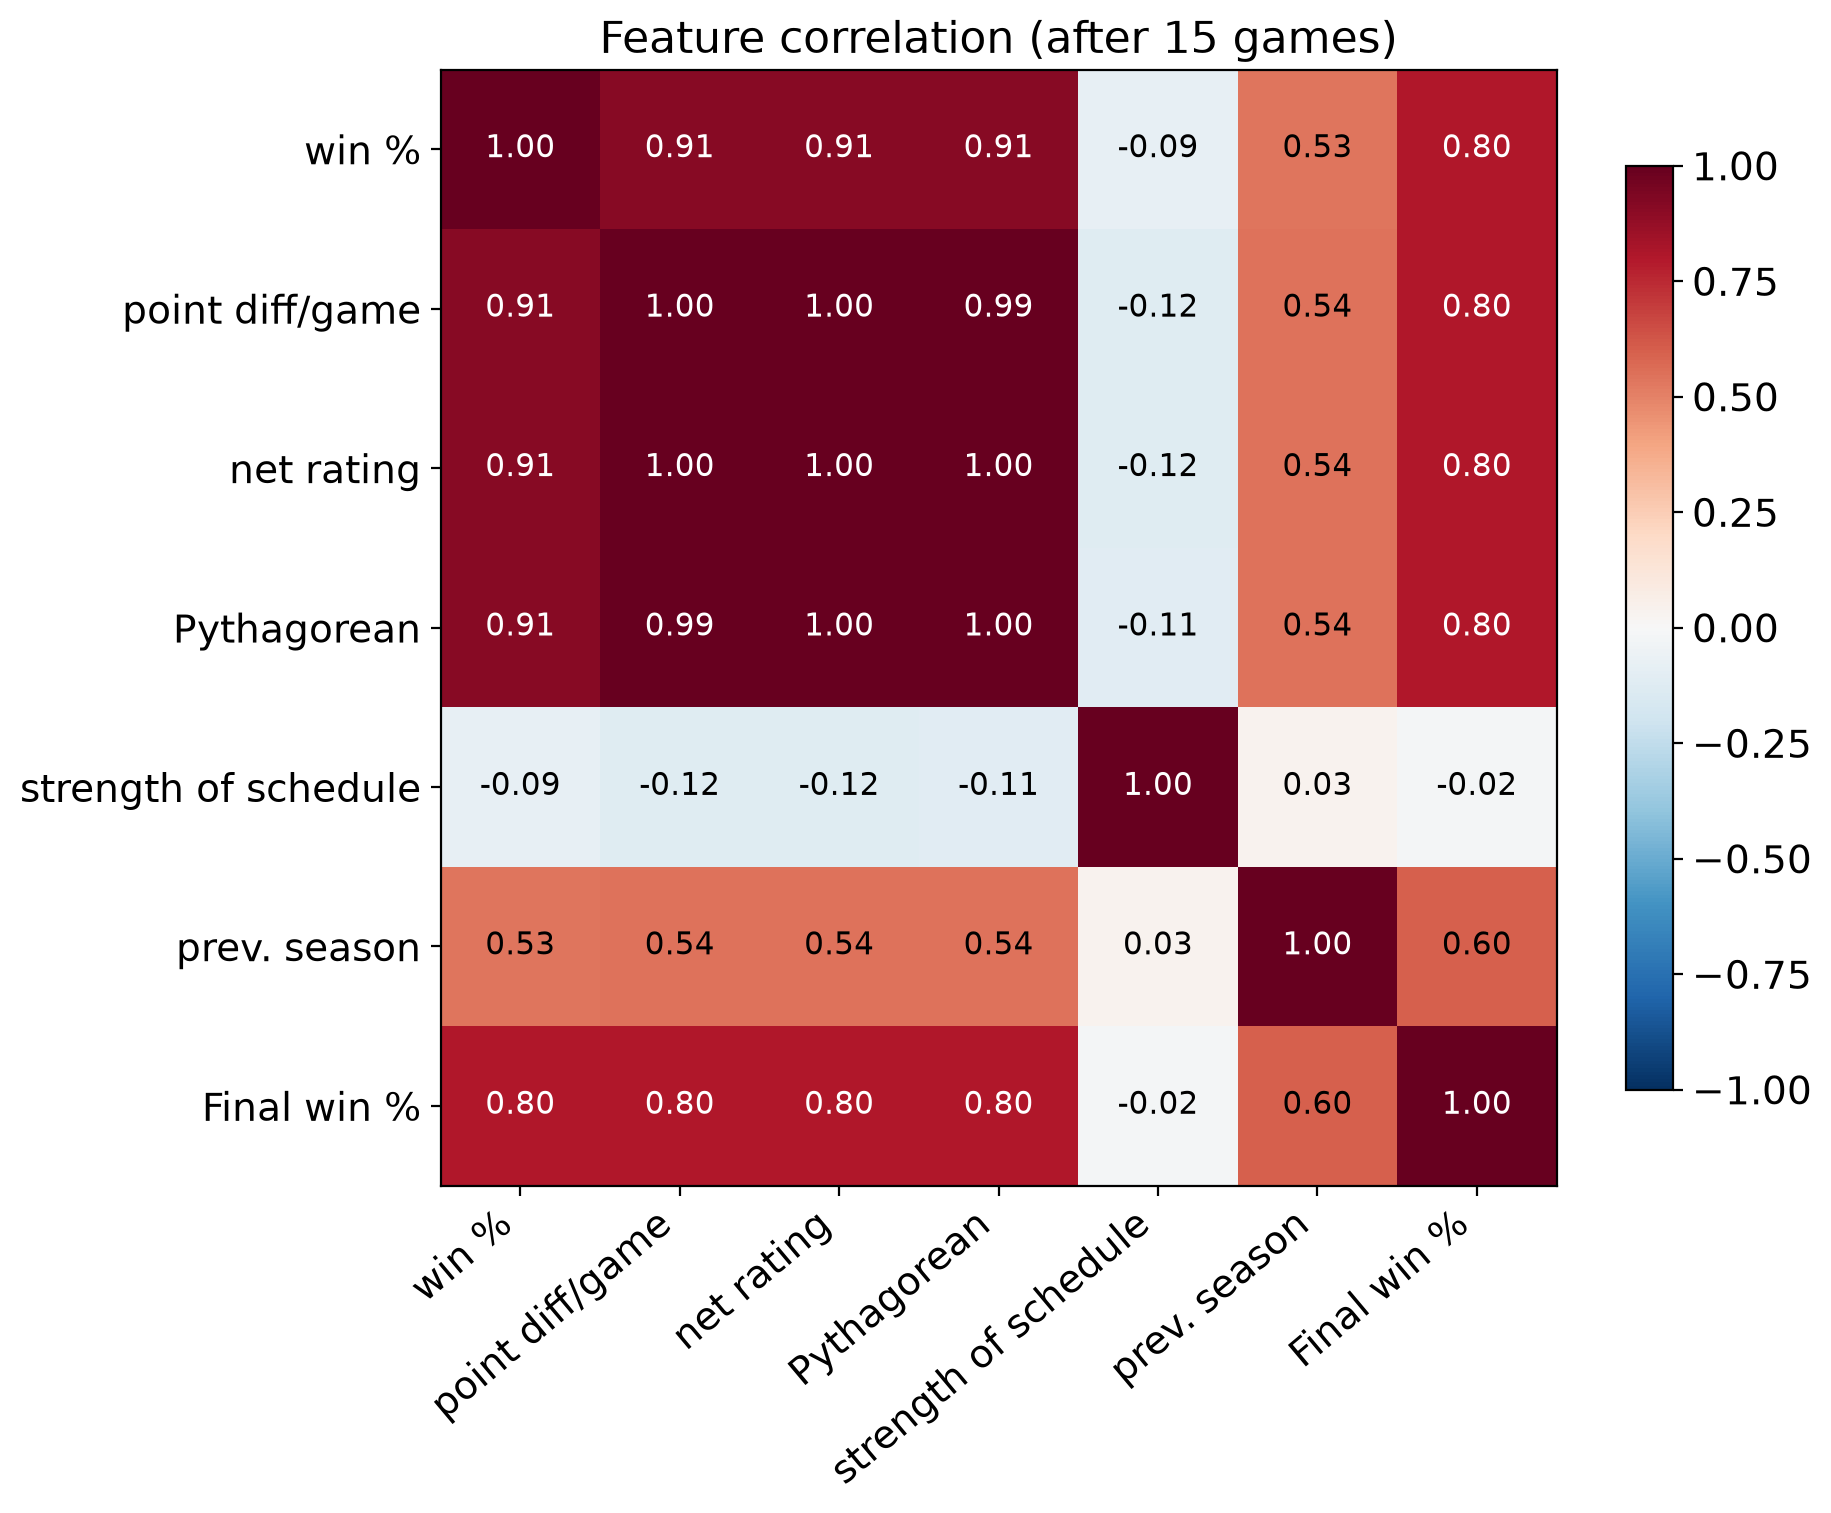
\includegraphics[width=0.92\columnwidth]{correlacao_features.png}}
\caption{Pearson correlation between features after 15 games and the final winning percentage (480 historical team-seasons).}
\label{fig:corr}
\end{figure}

%=====================================================================
\section{Method}
\subsection{Why shrinkage}
Fig.~\ref{fig:rtm} plots the final winning percentage against the winning percentage after 15 games. The least-squares slope is 0.63 and the line crosses $y=x$ near 0.500: each point above or below .500 after 15 games is worth only about 63\% of a point at the end of the season. The standard deviation of the win \% falls from 0.190 after 15 games to 0.151 at the end of the season. A good predictor must therefore \emph{shrink} early records toward the mean, which is precisely what regression models learn, and the remaining question is how to combine several noisy, collinear signals.

\begin{figure}[t]
\centerline{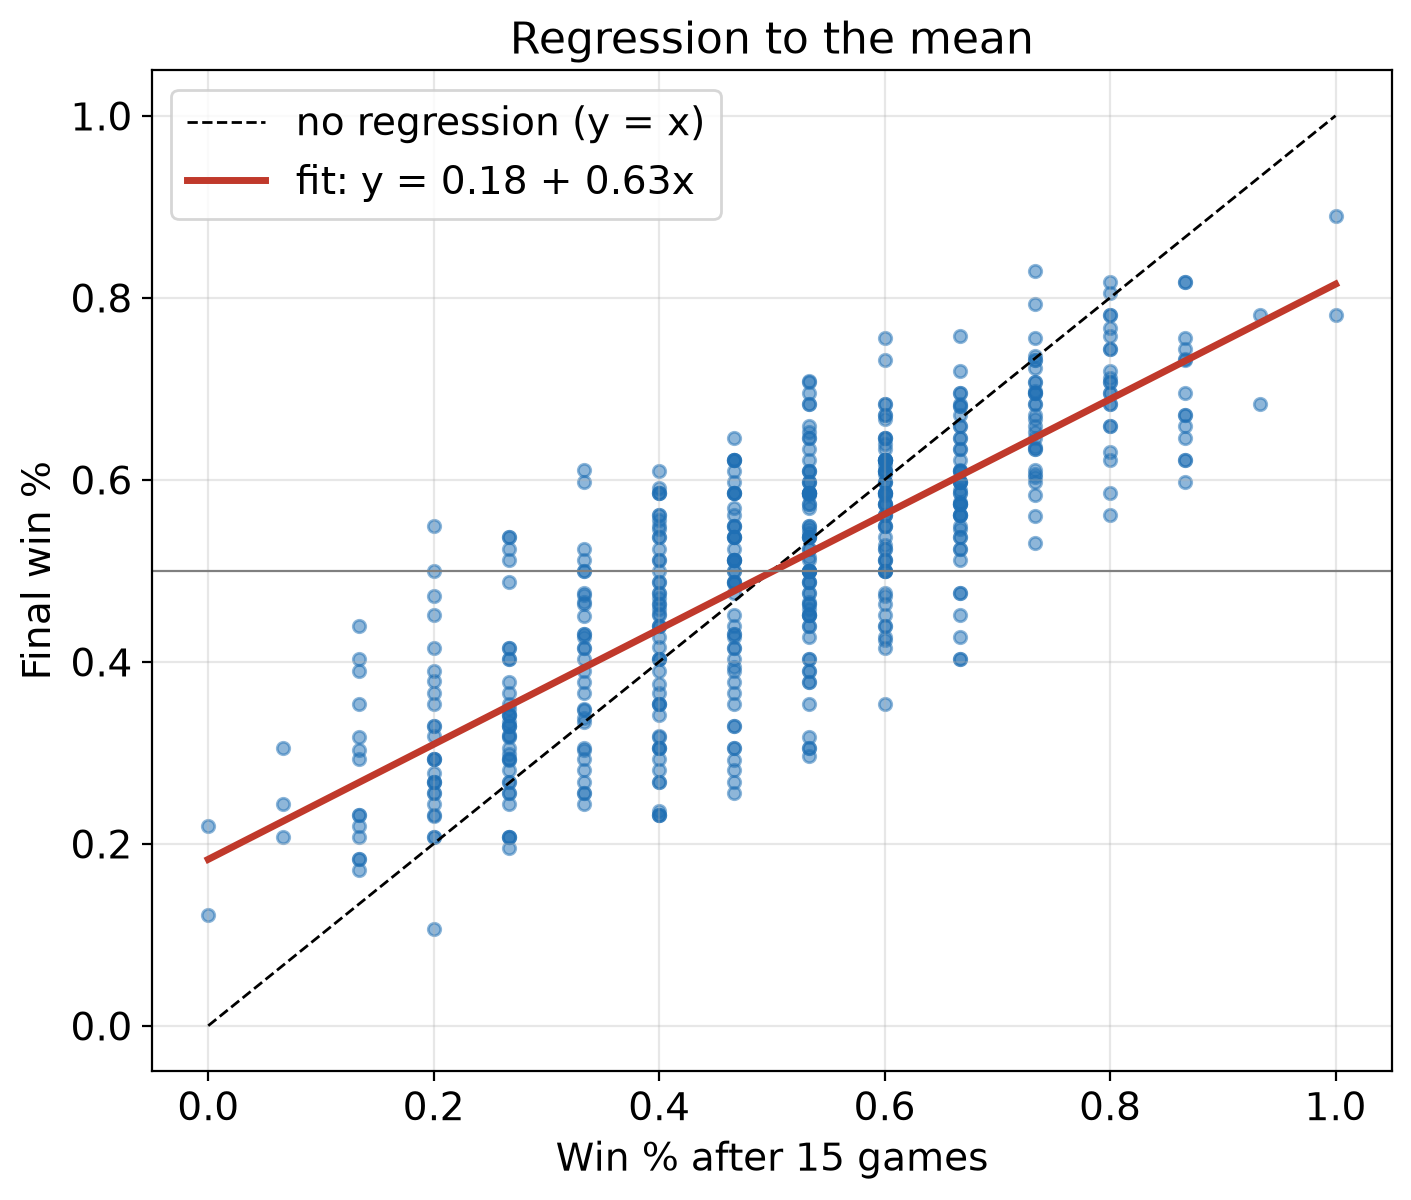
\includegraphics[width=0.85\columnwidth]{regressao_a_media.png}}
\caption{Regression to the mean: final win \% versus win \% after 15 games. The fitted slope (0.63) is well below the identity line.}
\label{fig:rtm}
\end{figure}

\subsection{Models}
We compare two baselines and four learned regressors:
\begin{itemize}
\item \textbf{Baseline A} keeps the current win \% ($\hat y = $ win \% after $N$ games).
\item \textbf{Baseline B} uses the Pythagorean expectation~\eqref{eq:pyth}.
\item \textbf{Linear regression (OLS)} on the six features.
\item \textbf{Ridge regression}~\cite{hoerl1970}, which minimizes
\begin{equation}
\sum_{i=1}^{n}\left(y_i-\beta_0-\mathbf{x}_i^{\top}\boldsymbol{\beta}\right)^2+\alpha\,\|\boldsymbol{\beta}\|_2^2 .
\label{eq:ridge}
\end{equation}
The $\ell_2$ penalty shrinks coefficients and, in particular, spreads weight across correlated predictors instead of giving them large coefficients of opposite signs~\cite{islr2021,esl2009}.
\item \textbf{Lasso}~\cite{tibshirani1996}, with an $\ell_1$ penalty that can set coefficients exactly to zero.
\item \textbf{Random forest}~\cite{breiman2001} with 500 trees, minimum leaf size 10 and 50\% of features per split, as a non-linear check.
\end{itemize}
All features are standardized inside a scikit-learn~\cite{sklearn} \texttt{Pipeline}, so scaling parameters are learned only on training folds.

\subsection{Validation protocol}
Team-seasons from the same season share league-wide conditions (rule changes, pace, the 2020 bubble), so the season is the natural grouping unit. We use (i) \textbf{leave-one-season-out} (LOSO) cross-validation, with 16 folds, and (ii) a \textbf{temporal holdout}, training on 2010--11 to 2022--23 and testing on 2023--24 to 2025--26. The regularization strength $\alpha$ of Ridge and Lasso is chosen by an \emph{inner} \texttt{GroupKFold} (5 folds, grouped by season) inside each outer training set, i.e.\ nested cross-validation. Because the inner validation curve is almost flat for small $\alpha$, we apply the \textbf{one-standard-error rule}~\cite{esl2009}: the largest $\alpha$ whose error is within one standard error of the minimum.

We report the MAE in wins (82-game scale) and the Spearman rank correlation between predicted and actual standings, computed per season and conference and then averaged. Among learned models whose LOSO MAE lies within one between-season standard error of the best, we select the most regularized one (preference order Ridge, Lasso, OLS, random forest).

\subsection{From forecasts to playoff odds}
\paragraph{Game model} Each team receives a rating $r$ equal to its predicted final win \%. For historical seasons we use the out-of-sample LOSO predictions, avoiding leakage. The probability that team $A$ beats team $B$ is modeled by a logistic regression, in the spirit of the Bradley--Terry model~\cite{bradley1952},
\begin{equation}
\mathrm{logit}\,P(A \text{ wins}) = b_{\Delta}\,(r_A - r_B) + b_{h}\,h,
\label{eq:logit}
\end{equation}
where $h=+1$ if $A$ plays at home and $-1$ otherwise; the intercept is omitted by symmetry. The model is fitted on all historical games played after the $N$-th game of both teams (30{,}790 team-game rows).

\paragraph{Rating uncertainty} A rating is itself an estimate. We decompose the variance of the LOSO residual of the final win \% into rating error and game-to-game luck,
\begin{equation}
\mathrm{Var}(y-\hat y) \approx f^2\sigma^2 + \frac{\overline{y(1-y)}\,(82-N)}{82^2}, \quad f=\frac{82-N}{82},
\label{eq:sigma}
\end{equation}
and solve for $\sigma$. In each simulation, every rating is perturbed by $\mathcal{N}(0,\sigma^2)$.

\paragraph{Monte Carlo} We simulate the 952 remaining 2026--27 games 10{,}000 times and add the results to each team's current record. Played and scheduled games add up to 80 per team: the last two games depend on the NBA Cup knockout stage, which is not yet scheduled, so they are simulated against a league-average opponent on a neutral court. Teams are ranked within each conference, and ties are broken at random. For each team we report expected wins, an 80\% interval (10th--90th percentiles) and the probabilities of finishing 1st--6th, 7th--10th and 11th--15th.

\paragraph{Backtest} To check calibration, we replay each historical season from the date on which the last team completed $N$ games, the same situation as in 2026--27, using LOSO ratings and refitting the game model~\eqref{eq:logit} and $\sigma$ without the tested season. We measure the coverage of the 80\% intervals and a three-class Brier score~\cite{brier1950}.

%=====================================================================
\section{Results}
\subsection{Model comparison}
Table~\ref{tab:models} summarizes both validation schemes. All four learned models cut the error of the naive baseline by about two wins (7.60 to 5.50--5.72 in LOSO) and improve the rank correlation. The differences among them are below one between-season standard error (0.25 wins). The temporal holdout tells the same story, so the models do not degrade on recent seasons. Fig.~\ref{fig:pvr} contrasts baseline A with Ridge: the baseline's vertical bands, one per possible record after 15 games, are compressed toward the diagonal.

\begin{table}[t]
\caption{Model comparison (MAE in wins on an 82-game scale; Spearman of conference standings)}
\begin{center}
\begin{tabular}{lcccc}
\toprule
 & \multicolumn{2}{c}{\textbf{LOSO (16 seasons)}} & \multicolumn{2}{c}{\textbf{Holdout 2023--26}} \\
\textbf{Model} & \textbf{MAE} & \textbf{Spearman} & \textbf{MAE} & \textbf{Spearman} \\
\midrule
Linear regression (OLS) & 5.50 & 0.785 & 5.22 & 0.867 \\
\textbf{Ridge} & 5.62 & 0.784 & 5.35 & 0.864 \\
Lasso & 5.68 & 0.788 & 5.45 & 0.877 \\
Random forest & 5.72 & 0.779 & 5.42 & 0.816 \\
Baseline: Pythagorean & 6.83 & 0.749 & 6.13 & 0.819 \\
Baseline: keep current win \% & 7.60 & 0.743 & 6.93 & 0.817 \\

\bottomrule
\end{tabular}
\label{tab:models}
\end{center}
\end{table}

\begin{figure*}[t]
\centerline{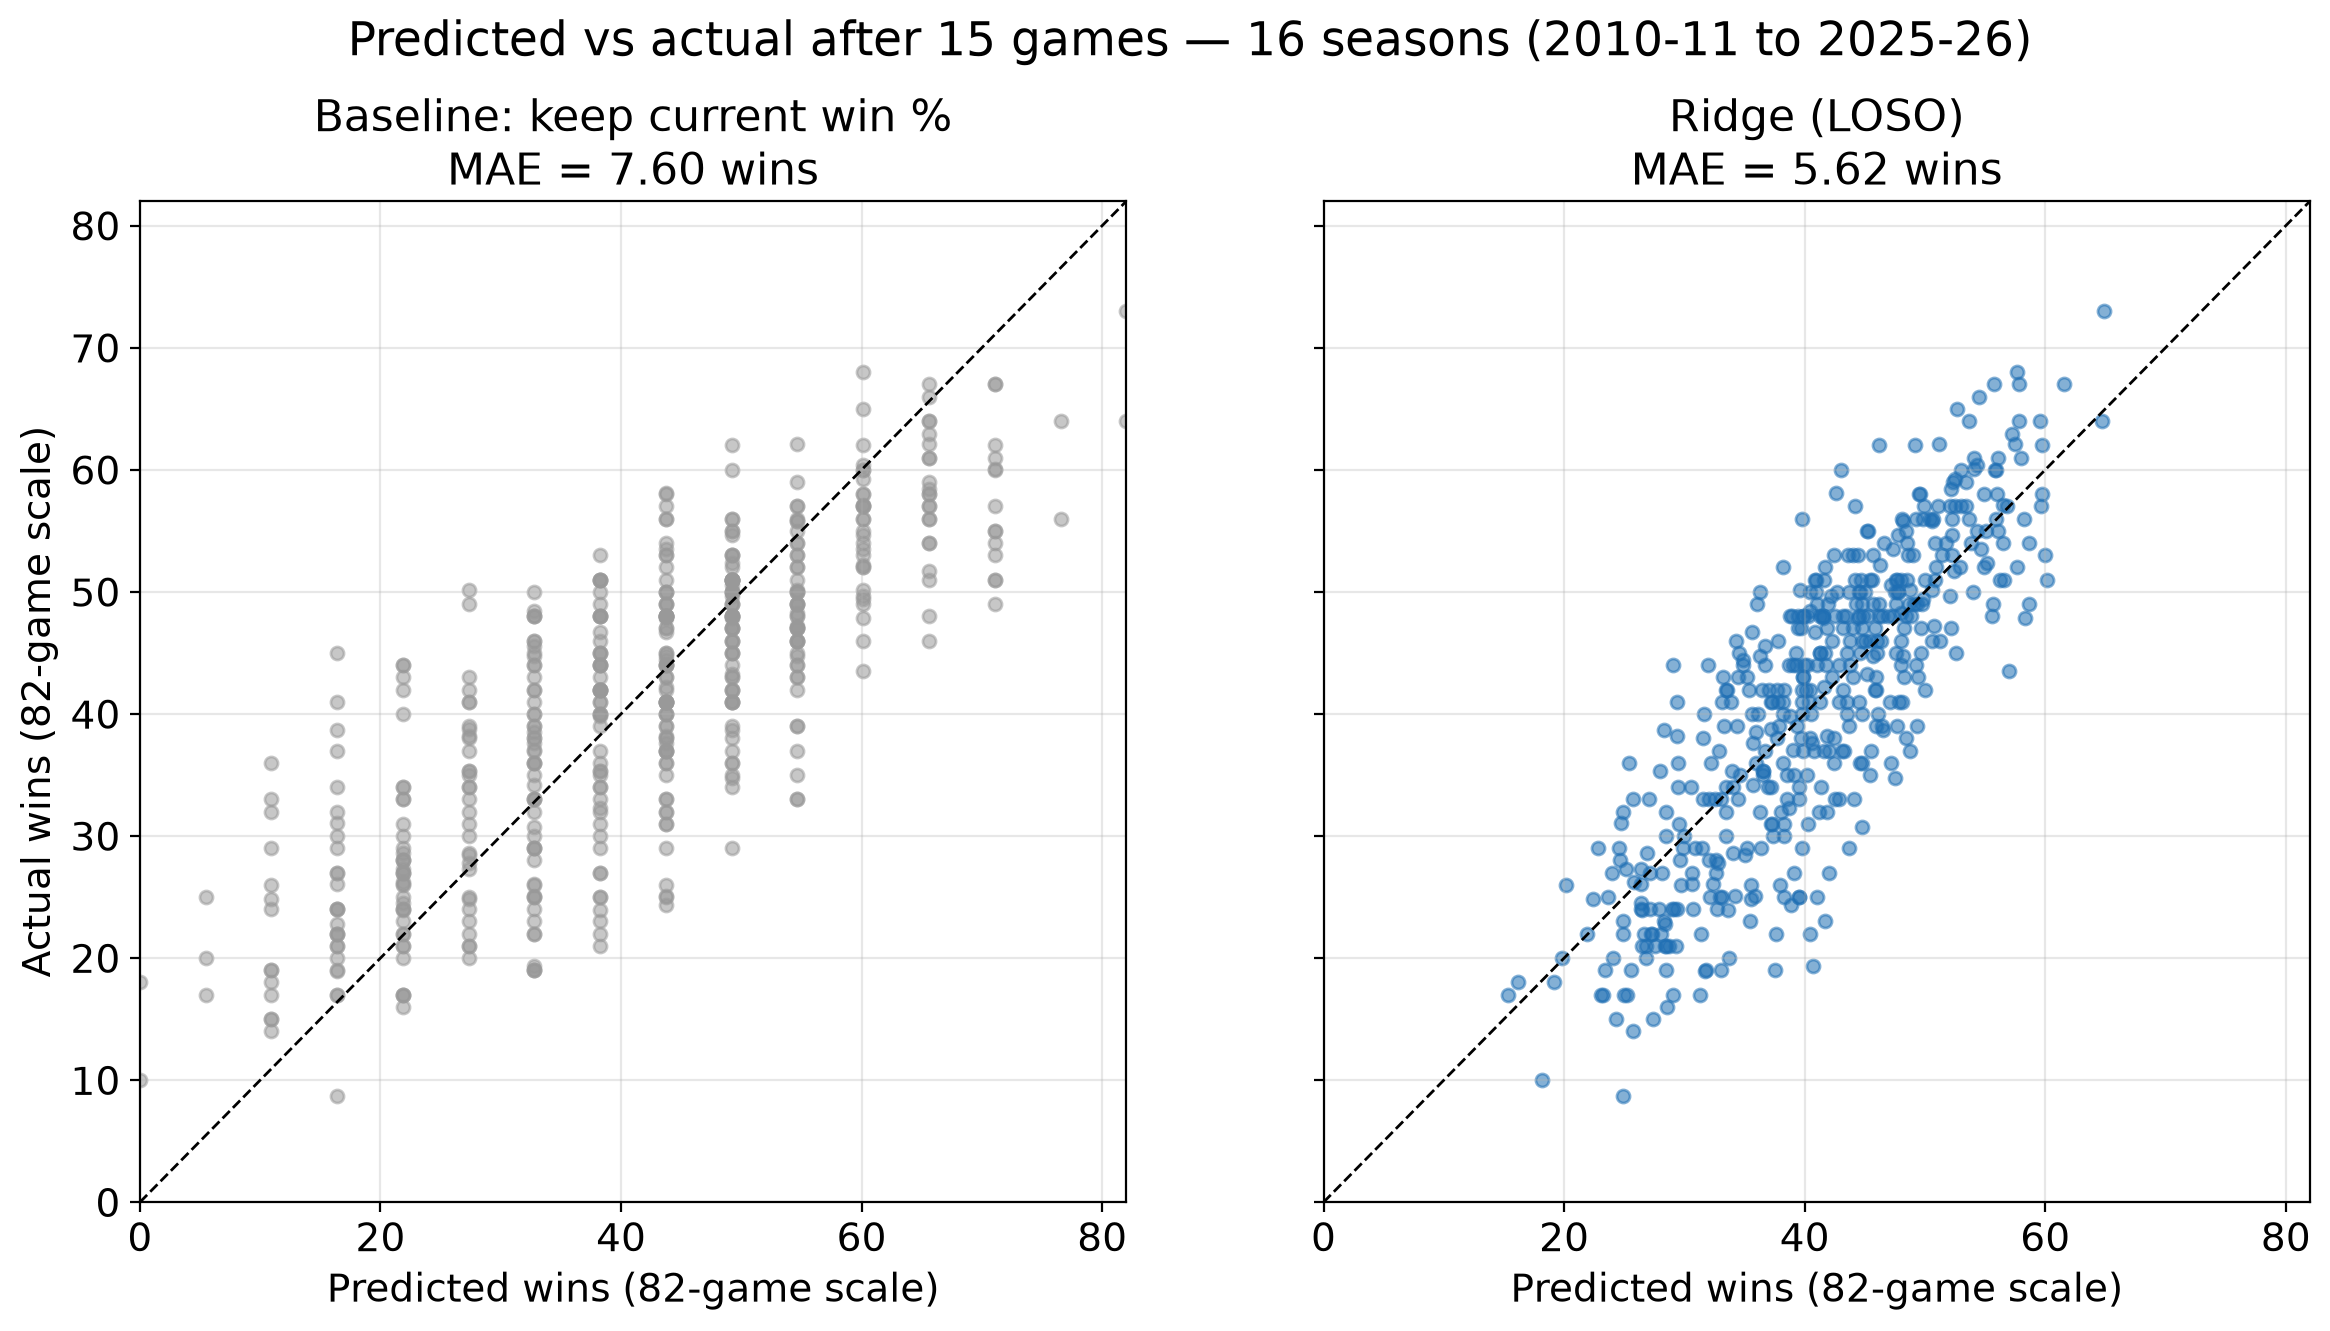
\includegraphics[width=0.85\textwidth]{previsto_vs_real.png}}
\caption{Predicted versus actual wins (82-game scale) for all 480 historical team-seasons, under leave-one-season-out validation. Left: baseline that keeps the win \% after 15 games. Right: Ridge.}
\label{fig:pvr}
\end{figure*}

\subsection{Why Ridge}
OLS has the lowest LOSO MAE (5.50 vs.\ 5.62), but the gap is within noise, while its coefficients are not interpretable (Table~\ref{tab:coefs}): point differential and net rating, correlated at 0.999, receive $+0.16$ and $-0.18$. Ridge, with $\alpha=100$ selected by the one-standard-error rule, distributes about the same weight ($\approx0.023$) across the three point-based features, keeps the early win \% and the previous season as relevant signals and gives strength of schedule almost no weight. The intercept equals 0.500, so predictions are shrunk toward the league mean. This is the stability we expect from $\ell_2$ regularization under multicollinearity~\cite{hoerl1970,islr2021}.

\begin{table}[t]
\caption{Standardized coefficients fitted on all 480 historical team-seasons}
\begin{center}
\begin{tabular}{lcc}
\toprule
\textbf{Feature} & \textbf{OLS} & \textbf{Ridge ($\alpha=100$)} \\
\midrule
Win \% & 0.053 & 0.036 \\
Point diff./game & 0.161 & 0.023 \\
Net rating & -0.180 & 0.022 \\
Pythagorean exp. & 0.075 & 0.024 \\
Strength of schedule & 0.007 & 0.006 \\
Prev. season win \% & 0.032 & 0.028 \\

\bottomrule
\end{tabular}
\label{tab:coefs}
\end{center}
\end{table}

\subsection{How many games are needed?}
Repeating the LOSO evaluation with features built from $N=5$ to $41$ games (Table~\ref{tab:sens}, Fig.~\ref{fig:sens}) shows that the gain of the model is largest when information is scarce: after 5 games, Ridge cuts the baseline error by 46\%, from 13.3 to 7.2 wins. After half a season ($N=41$), the two approaches nearly converge, because the record itself is no longer very noisy.

\begin{table}[t]
\caption{Sensitivity to the number of games $N$ (LOSO)}
\begin{center}
\begin{tabular}{ccccc}
\toprule
$N$ & \textbf{Baseline MAE} & \textbf{Ridge MAE} & \textbf{Gain} & \textbf{Ridge Spearman} \\
\midrule
5 & 13.29 & 7.18 & 46\% & 0.655 \\
10 & 9.09 & 6.25 & 31\% & 0.728 \\
15 & 7.60 & 5.62 & 26\% & 0.784 \\
20 & 6.64 & 5.34 & 20\% & 0.808 \\
25 & 6.15 & 4.94 & 20\% & 0.816 \\
30 & 5.31 & 4.61 & 13\% & 0.855 \\
41 & 3.94 & 3.60 & 9\% & 0.902 \\

\bottomrule
\end{tabular}
\label{tab:sens}
\end{center}
\end{table}

\begin{figure}[t]
\centerline{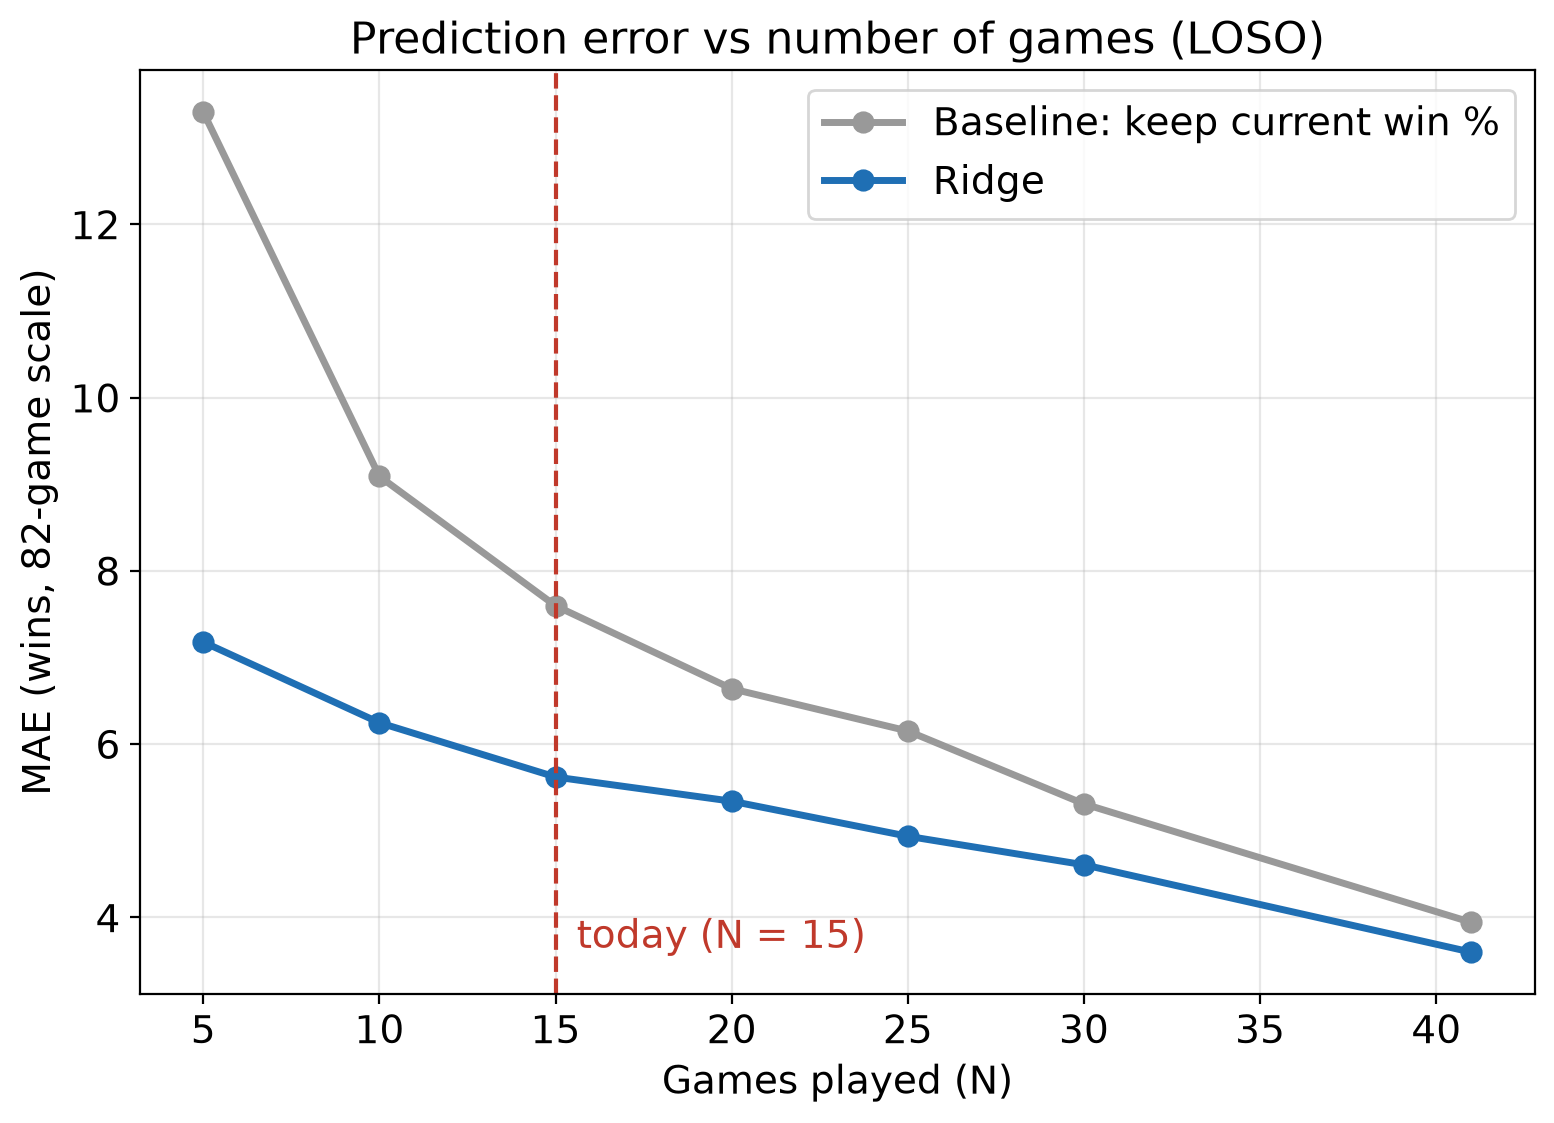
\includegraphics[width=0.9\columnwidth]{sensibilidade_n.png}}
\caption{Leave-one-season-out MAE as a function of the number of games used to build the features.}
\label{fig:sens}
\end{figure}

\subsection{Simulation}
The fitted game model has $b_{\Delta}=4.35$ and $b_h=0.32$, i.e.\ a 57.9\% home win probability between equal teams; its accuracy on the training games is 64.3\% (log-loss 0.629). Eq.~\eqref{eq:sigma} gives $\sigma=0.085$. In the out-of-sample backtest, the 80\% intervals contain the actual number of wins in 81.0\% of the 480 team-seasons, and the three-class Brier score is 0.421, against 0.658 for constant probabilities (6/15, 4/15, 5/15). Fig.~\ref{fig:calib} shows that predicted and observed frequencies follow the diagonal closely.

\begin{figure}[t]
\centerline{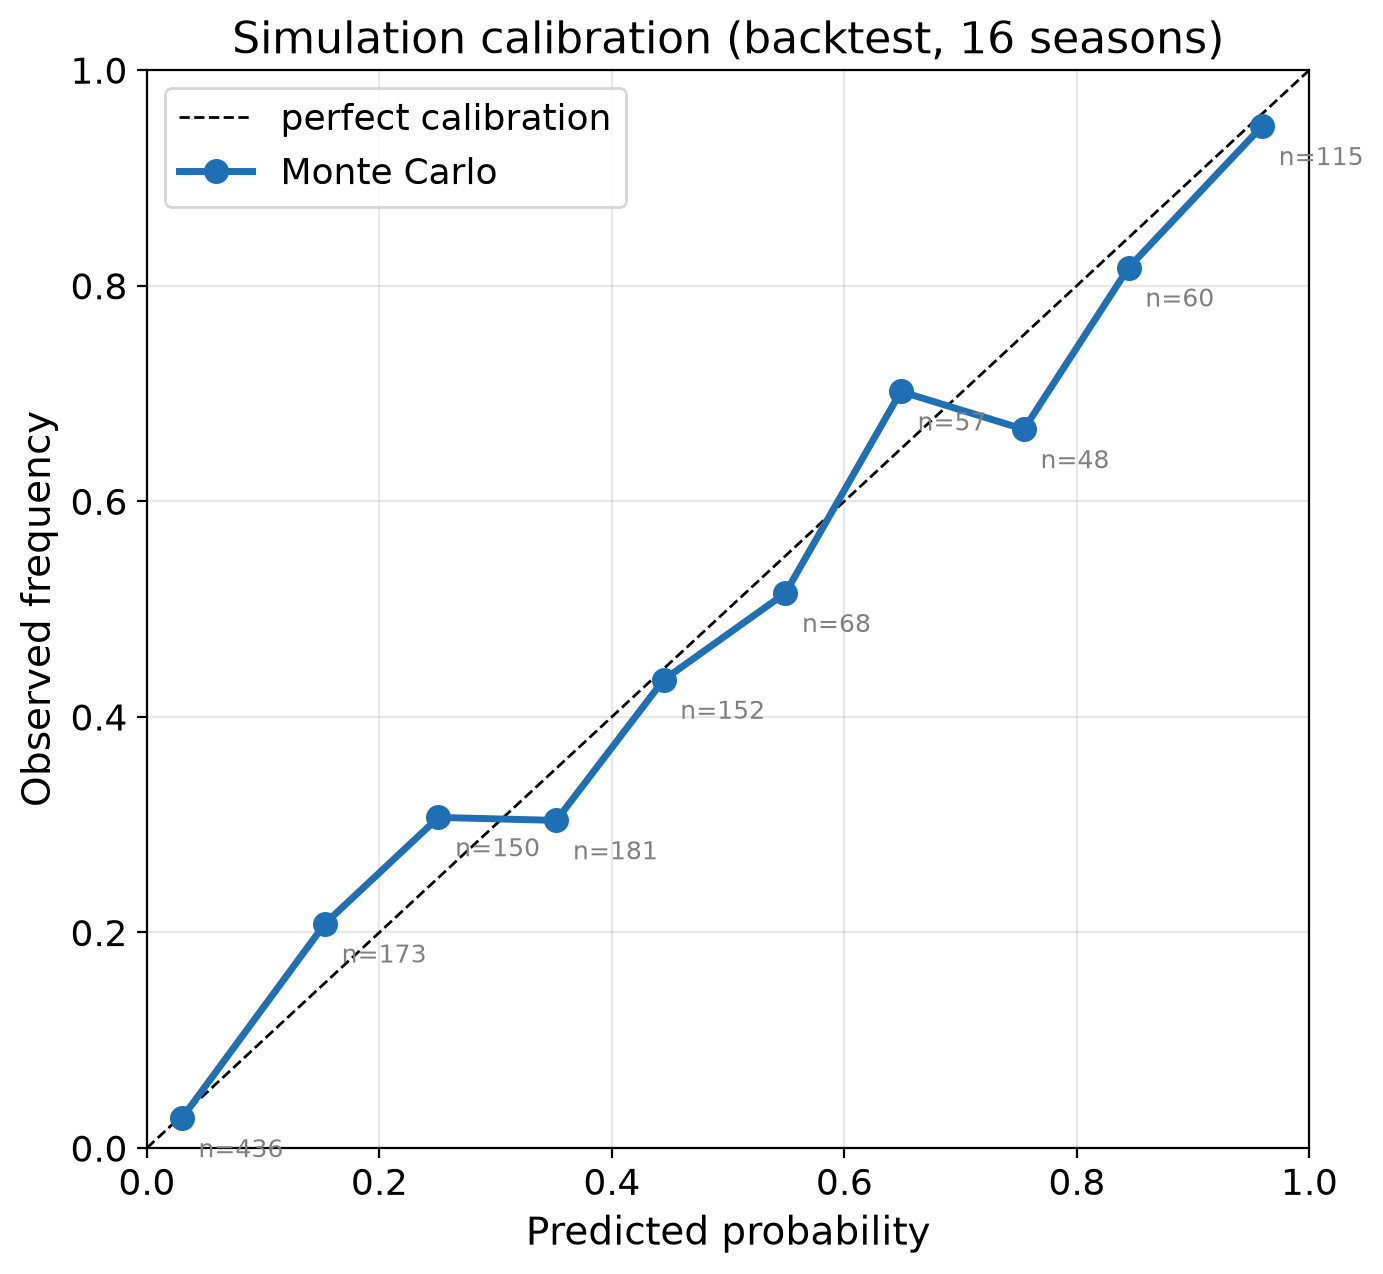
\includegraphics[width=0.8\columnwidth]{calibracao_simulacao.png}}
\caption{Calibration of the simulated probabilities of top six, play-in and out in the out-of-sample backtest (16 seasons, bins of width 0.1; $n$ = number of team-class pairs).}
\label{fig:calib}
\end{figure}

\subsection{2026--27 projection}
Table~\ref{tab:proj} and Fig.~\ref{fig:heat} show the projection as of November 22, 2026. Boston (97\% top six) and San Antonio (95\%) are the clearest favorites. The model also tempers hot starts: Philadelphia is 14--3 but projects to 52.4 wins, since its point differential is modest, and Memphis, 12--5 after a 25-win season, has only a 48\% chance of a top-six finish. At the bottom, Sacramento and Utah have less than a 1\% chance of reaching even the play-in.

\begin{table*}[t]
\caption{2026--27 projection (10{,}000 simulations, as of Nov.\ 22, 2026): current record, expected wins, 80\% interval and probabilities (\%) of top six, play-in and out}
\begin{center}
\footnotesize
\setlength{\tabcolsep}{4.2pt}
\begin{tabular}{rlccccccrlcccccc}
\toprule
\multicolumn{8}{c}{\textbf{Eastern Conference}} & \multicolumn{8}{c}{\textbf{Western Conference}} \\
\cmidrule(lr){1-8}\cmidrule(lr){9-16}
\# & Team & W--L & E[W] & 80\% int. & Top 6 & Play-in & Out & \# & Team & W--L & E[W] & 80\% int. & Top 6 & Play-in & Out \\
\midrule
1 & BOS & 11--6 & 55.8 & 48--63 & 97 & 3 & 0 & 1 & SAS & 14--3 & 58.9 & 51--66 & 95 & 5 & 0 \\
2 & DET & 10--6 & 53.6 & 46--61 & 94 & 6 & 0 & 2 & LAL & 14--3 & 55.8 & 48--63 & 86 & 14 & 0 \\
3 & PHI & 14--3 & 52.4 & 44--60 & 90 & 9 & 0 & 3 & HOU & 12--5 & 54.5 & 47--62 & 82 & 17 & 1 \\
4 & NYK & 11--6 & 50.9 & 43--59 & 86 & 13 & 0 & 4 & MIN & 12--5 & 54.3 & 46--62 & 81 & 18 & 1 \\
5 & ATL & 11--6 & 46.5 & 38--55 & 67 & 32 & 1 & 5 & OKC & 10--7 & 50.5 & 43--58 & 61 & 36 & 3 \\
6 & CLE & 9--8 & 45.7 & 37--54 & 62 & 36 & 2 & 6 & POR & 10--6 & 50.2 & 42--58 & 59 & 38 & 3 \\
7 & MIA & 10--6 & 45.6 & 37--54 & 61 & 37 & 2 & 7 & MEM & 12--5 & 48.5 & 40--57 & 48 & 46 & 6 \\
8 & TOR & 6--10 & 38.1 & 30--47 & 19 & 65 & 16 & 8 & DEN & 10--5 & 48.5 & 40--57 & 47 & 47 & 6 \\
9 & ORL & 7--9 & 38.0 & 29--47 & 18 & 65 & 16 & 9 & GSW & 9--8 & 43.2 & 35--51 & 19 & 60 & 21 \\
10 & IND & 5--12 & 30.7 & 23--39 & 3 & 41 & 56 & 10 & PHX & 8--7 & 41.8 & 33--50 & 14 & 57 & 29 \\
11 & CHI & 4--12 & 28.2 & 20--36 & 1 & 28 & 71 & 11 & DAL & 10--7 & 39.7 & 32--48 & 8 & 51 & 42 \\
12 & CHA & 4--11 & 27.8 & 20--36 & 1 & 26 & 73 & 12 & LAC & 4--11 & 29.5 & 21--38 & 0 & 8 & 92 \\
13 & WAS & 7--11 & 27.7 & 20--35 & 0 & 24 & 76 & 13 & NOP & 5--13 & 26.6 & 19--34 & 0 & 3 & 97 \\
14 & BKN & 3--12 & 24.0 & 17--32 & 0 & 11 & 89 & 14 & UTA & 3--15 & 23.2 & 16--31 & 0 & 1 & 99 \\
15 & MIL & 1--16 & 20.2 & 13--28 & 0 & 3 & 97 & 15 & SAC & 2--14 & 19.7 & 13--27 & 0 & 0 & 100 \\

\bottomrule
\end{tabular}
\label{tab:proj}
\end{center}
\end{table*}

\begin{figure*}[t]
\centerline{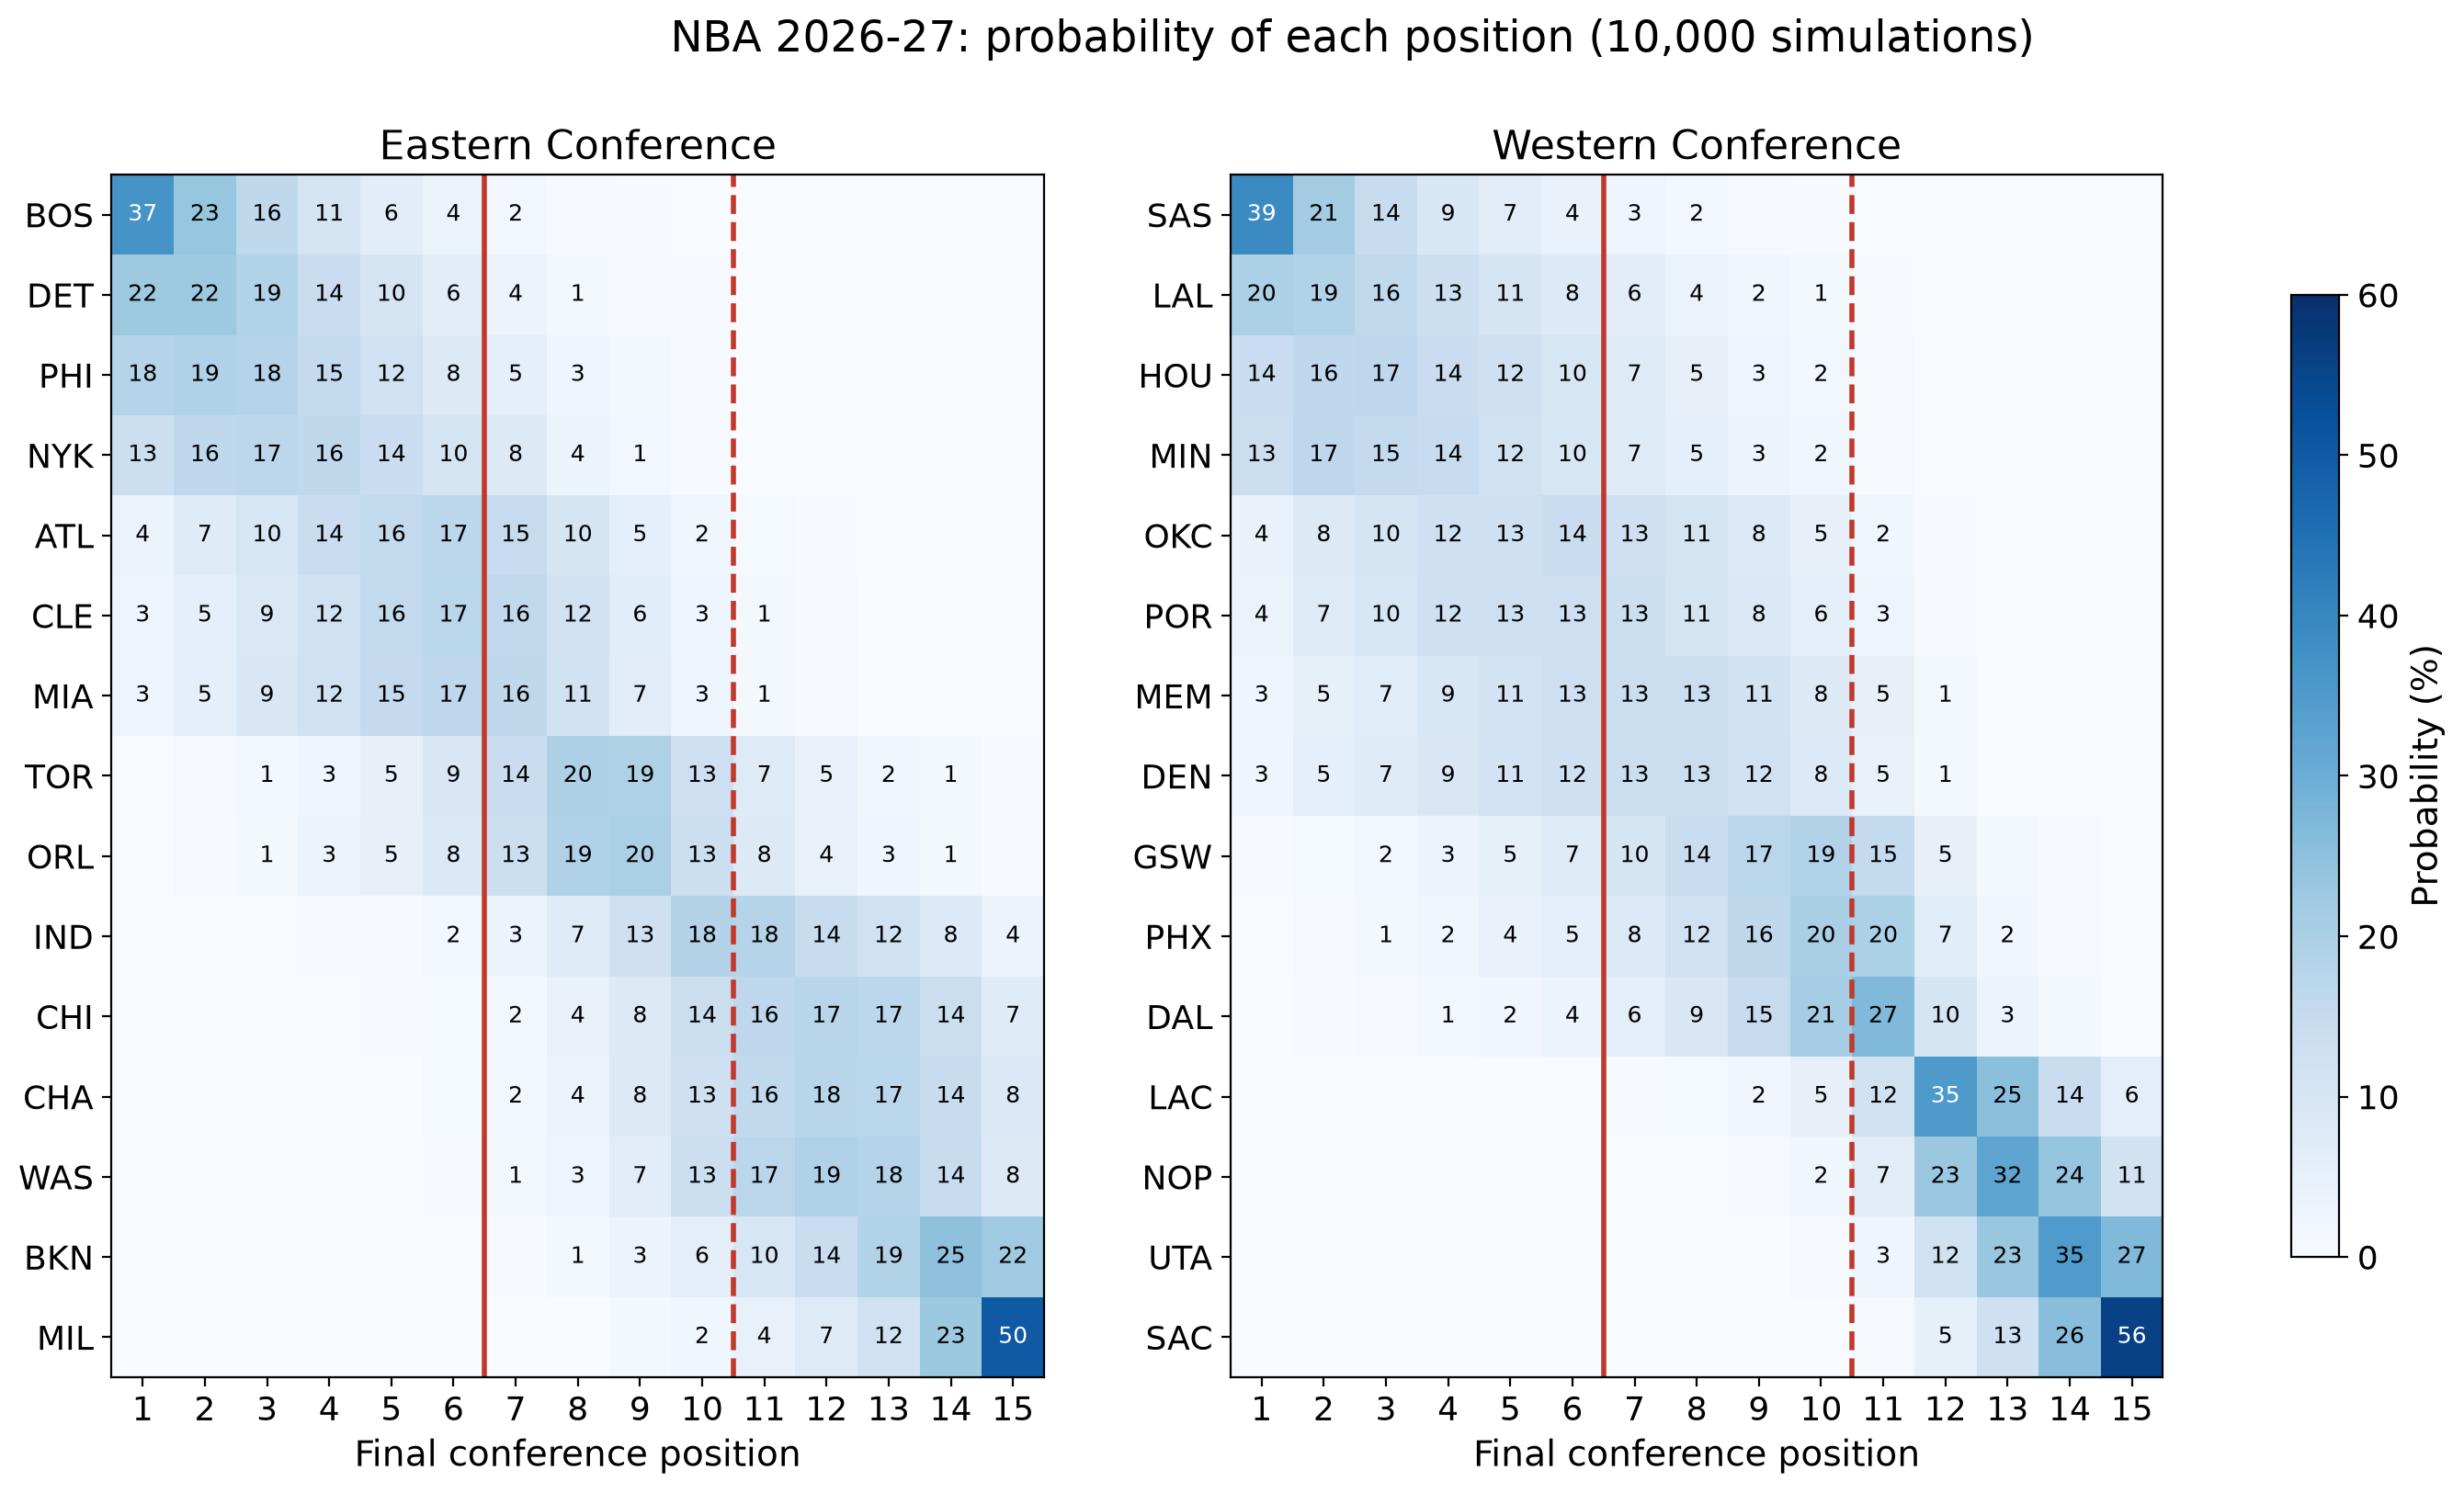
\includegraphics[width=0.92\textwidth]{heatmap_posicoes.png}}
\caption{Probability (\%) of each final conference position in 2026--27. Solid line: top-six cutoff; dashed line: play-in cutoff.}
\label{fig:heat}
\end{figure*}

%=====================================================================
\section{Discussion}
The main finding is that \emph{how} early records are shrunk matters more than \emph{which} learner is used: once a model is allowed to regress the record toward the mean and combine it with point differential and the previous season, OLS, Ridge, Lasso and random forests are statistically indistinguishable, and all beat the naive baselines by a wide margin. The random forest does not improve on linear models, which is consistent with an almost linear relationship (Fig.~\ref{fig:rtm}) and a small sample (480 rows). Ridge was preferred not for accuracy but for stability: its coefficients are interpretable and robust to the near-exact collinearity among point-based features, which is the textbook motivation for $\ell_2$ regularization. Note that the regression to the mean itself is captured by any linear model, through a slope below one and an intercept at 0.500; the penalty adds coefficient stability, not extra shrinkage toward 0.500.

The Pythagorean baseline beats the raw record, confirming that point differential is a less noisy signal of strength than wins and losses. Strength of schedule after 15 games carries almost no information, probably because opponents' records are themselves noisy at that point.

The backtest is the strongest evidence that the probabilities can be trusted: intervals have their nominal coverage and the calibration curve tracks the diagonal. Without the rating-uncertainty term, the simulation would treat the forecasts as exact and the intervals would be too narrow.

\paragraph*{Limitations} (i) With 15 games, even the best model errs by about 5.6 wins on average; a single injury can move a team more than that. (ii) Injuries, trades and roster changes are not modeled; ratings depend only on results. (iii) Ratings are static: they use only the first 15 games, to match training, so the 16th to 18th games of teams that have played them count as wins but do not update ratings. (iv) Ties are broken at random instead of using the official NBA tiebreakers. (v) The two NBA Cup games not yet scheduled are simulated against an average opponent, and neutral-site games are treated as regular home games. (vi) The home-court effect is assumed constant across seasons, including the 2020--21 season played largely without fans.

%=====================================================================
\section{Conclusion}
Fifteen games are not a season, but they are not useless either. A regularized linear model built on six simple features reduces the error of the naive ``current record'' forecast by a quarter (7.6 to 5.6 wins), and by nearly half after only five games. Combined with a logistic game model, rating uncertainty and Monte Carlo simulation, it produces calibrated probabilities of top-six, play-in and out finishes for the 2026--27 season. Natural extensions are player-level information (injuries, minutes, trades), ratings updated game by game and the official tiebreaking rules.

%=====================================================================
\section*{Author Contributions}
[To be completed by the authors. Example: A1 defined the research question and the project plan, collected the data and wrote the article; A2 implemented the models and the simulation, produced the figures and prepared the lightning talk. All authors reviewed the final version.]

\section*{Declaration of AI Use}
Claude (Anthropic), through the Claude Code tool, was used in this project to implement and debug the Python code (data collection, features, models, simulation and figures) following a phased plan written by the authors; to review the methodology, which led to the one-standard-error rule for $\alpha$ and to the out-of-sample backtest of the simulation; and to draft this article and the presentation slides in English and Portuguese. The authors defined the research question, the data source, the features, the models and the validation protocol, checked the results by running the notebook, and are responsible for all content. [Authors: adjust this statement to reflect your actual use.]

\begin{thebibliography}{00}
\bibitem{efron1975} B. Efron and C. Morris, ``Data analysis using Stein's estimator and its generalizations,'' \textit{J. Amer. Statist. Assoc.}, vol. 70, no. 350, pp. 311--319, 1975.
\bibitem{efron1977} B. Efron and C. Morris, ``Stein's paradox in statistics,'' \textit{Scientific American}, vol. 236, no. 5, pp. 119--127, 1977.
\bibitem{hoerl1970} A. E. Hoerl and R. W. Kennard, ``Ridge regression: biased estimation for nonorthogonal problems,'' \textit{Technometrics}, vol. 12, no. 1, pp. 55--67, 1970.
\bibitem{tibshirani1996} R. Tibshirani, ``Regression shrinkage and selection via the lasso,'' \textit{J. Roy. Statist. Soc. B}, vol. 58, no. 1, pp. 267--288, 1996.
\bibitem{breiman2001} L. Breiman, ``Random forests,'' \textit{Machine Learning}, vol. 45, no. 1, pp. 5--32, 2001.
\bibitem{metropolis1949} N. Metropolis and S. Ulam, ``The Monte Carlo method,'' \textit{J. Amer. Statist. Assoc.}, vol. 44, no. 247, pp. 335--341, 1949.
\bibitem{nbaapi} S. Patel \textit{et al.}, ``nba\_api: an API client package to access the APIs for NBA.com,'' 2024. [Online]. Available: \url{https://github.com/swar/nba_api}
\bibitem{kubatko2007} J. Kubatko, D. Oliver, K. Pelton, and D. T. Rosenbaum, ``A starting point for analyzing basketball statistics,'' \textit{J. Quant. Anal. Sports}, vol. 3, no. 3, 2007.
\bibitem{islr2021} G. James, D. Witten, T. Hastie, and R. Tibshirani, \textit{An Introduction to Statistical Learning}, 2nd ed. New York: Springer, 2021.
\bibitem{esl2009} T. Hastie, R. Tibshirani, and J. Friedman, \textit{The Elements of Statistical Learning}, 2nd ed. New York: Springer, 2009.
\bibitem{sklearn} F. Pedregosa \textit{et al.}, ``Scikit-learn: machine learning in Python,'' \textit{J. Mach. Learn. Res.}, vol. 12, pp. 2825--2830, 2011.
\bibitem{bradley1952} R. A. Bradley and M. E. Terry, ``Rank analysis of incomplete block designs: I. The method of paired comparisons,'' \textit{Biometrika}, vol. 39, no. 3/4, pp. 324--345, 1952.
\bibitem{brier1950} G. W. Brier, ``Verification of forecasts expressed in terms of probability,'' \textit{Monthly Weather Review}, vol. 78, no. 1, pp. 1--3, 1950.
\end{thebibliography}

\end{document}
